\documentclass[12pt, a4paper]{article}

\usepackage[utf8]{inputenc}
\usepackage[english, russian]{babel}
\usepackage{fancyhdr}
\usepackage{amsmath}
\usepackage{amsthm}
\usepackage{float}
\usepackage{graphicx}
\graphicspath{ {./} }
\usepackage{tabularx}
\newcolumntype{L}{>{\raggedright\arraybackslash}X}
\usepackage{pgfplots}
\usepackage{float}
\usepackage{xcolor}
\usepackage{hyperref}
\usepackage{multirow}
\usepackage{diagbox}
\pgfplotsset{width=\textwidth*0.8, compat=1.13}

\usepgfplotslibrary{external}
\usepgfplotslibrary{fillbetween}
\usepgfplotslibrary{statistics}
\usetikzlibrary{patterns.meta}


\graphicspath{{./}}
\newcommand{\Mod}[1]{\ \mathrm{mod}\ #1}

\usepackage[a4paper, margin=1.5cm]{geometry}

\usepackage{titlesec}
\titlelabel{\thetitle.\quad}

\pagestyle{plain}

\fancypagestyle{firstpage}{%
  \chead{
  МИНИСТЕРСТВО НАУКИ И ВЫСШЕГО ОБРАЗОВАНИЯ РОССИЙСКОЙ ФЕДЕРАЦИИ 
ФЕДЕРАЛЬНОЕ ГОСУДАРСТВЕННОЕ АВТОНОМНОЕ  
ОБРАЗОВАТЕЛЬНОЕ УЧРЕЖДЕНИЕ ВЫСШЕГО ОБРАЗОВАНИЯ\bigskip

«Национальный исследовательский университет ИТМО»\bigskip

ФИЗИЧЕСКИЙ ФАКУЛЬТЕТ 
}
\fancyfoot[CO]{Санкт-Петербург, 2023}%
}



\definecolor{aqua}{HTML}{003844}
\definecolor{peri}{HTML}{5EB1BF}
\definecolor{royal_blue}{HTML}{0A2463}
\definecolor{periwinkle}{HTML}{D8DCFF}
\definecolor{cerulean}{HTML}{247BA0}
\definecolor{bloodred}{HTML}{690500}
\definecolor{imperial_red}{HTML}{FB3640}
\definecolor{purple}{HTML}{511730}
\definecolor{tangerine}{HTML}{FFA781}

\definecolor{blue1}{HTML}{142459}
\definecolor{blue2}{HTML}{176BA0}
\definecolor{blue3}{HTML}{19AADE}
\definecolor{blue4}{HTML}{1AC936}
\definecolor{blue5}{HTML}{1DE4BD}
\definecolor{blue6}{HTML}{6DF0D2}

\definecolor{pink1}{HTML}{29066B}
\definecolor{pink2}{HTML}{7D3AC1}
\definecolor{pink3}{HTML}{AF4BCE}
\definecolor{pink4}{HTML}{DB4CB2}
\definecolor{pink5}{HTML}{EB548C}
\definecolor{pink6}{HTML}{EA7369}
\newtheorem*{task}{Условие}
\newtheorem*{finish}{Заключение}

\counterwithin{figure}{section}

%\tikzexternalize
\begin{document}
\newgeometry{top=1.6cm,bottom=1.6cm, left = 1.2cm, right = 1.2cm}

\topskip0pt
\vspace*{0.25\textheight}
\begin{center}
\textbf{\LARGE РАБОЧИЙ ПРОТОКОЛ И ОТЧЁТ }

\LARGE по лабораторной работе №1.14

\LARGE <<Изучение колебаний струны>>

\end{center}
\vspace*{5cm}
\begin{flushright}
\begin{minipage}{.33\linewidth}
\textit{\textbf{Выполнил:}}\\
Хороших Дмитрий - P3217\\
\textit{\textbf{Преподаватель:}}\\
Хуснутдинова Наира\\ Рустемовна
\end{minipage}
\end{flushright}


\thispagestyle{firstpage}
\newpage
\tableofcontents

\restoregeometry
\section{Введение}
\begin{enumerate}
\item Цель работы:

Пронаблюдать поперечные стоячие волны на тонкой натянутой струне и экспериментально определить зависимость собственных частот поперечных колебаний от номера гармоники и силы натяжения струны.
\item Задачи:
	\begin{enumerate}
		\item[1.]  Измерить значения резонансных частот колебаний струны в режиме формирования стоячих волн. Рассчитать значения скорости волны и погонной плотности струны при известной силе её натяжения.
		\item[2.] Провести прямое измерение массы и длины струны, непосредственно определить её погонную плотность.
		\item[3.] Сравнить полученные значения погонных плотностей $\rho_{l}$.
	\end{enumerate}
		
\item Объект исследования:

Колебаемая вибратором струна в установке.

\item Схема установки:
\begin{figure}[H]
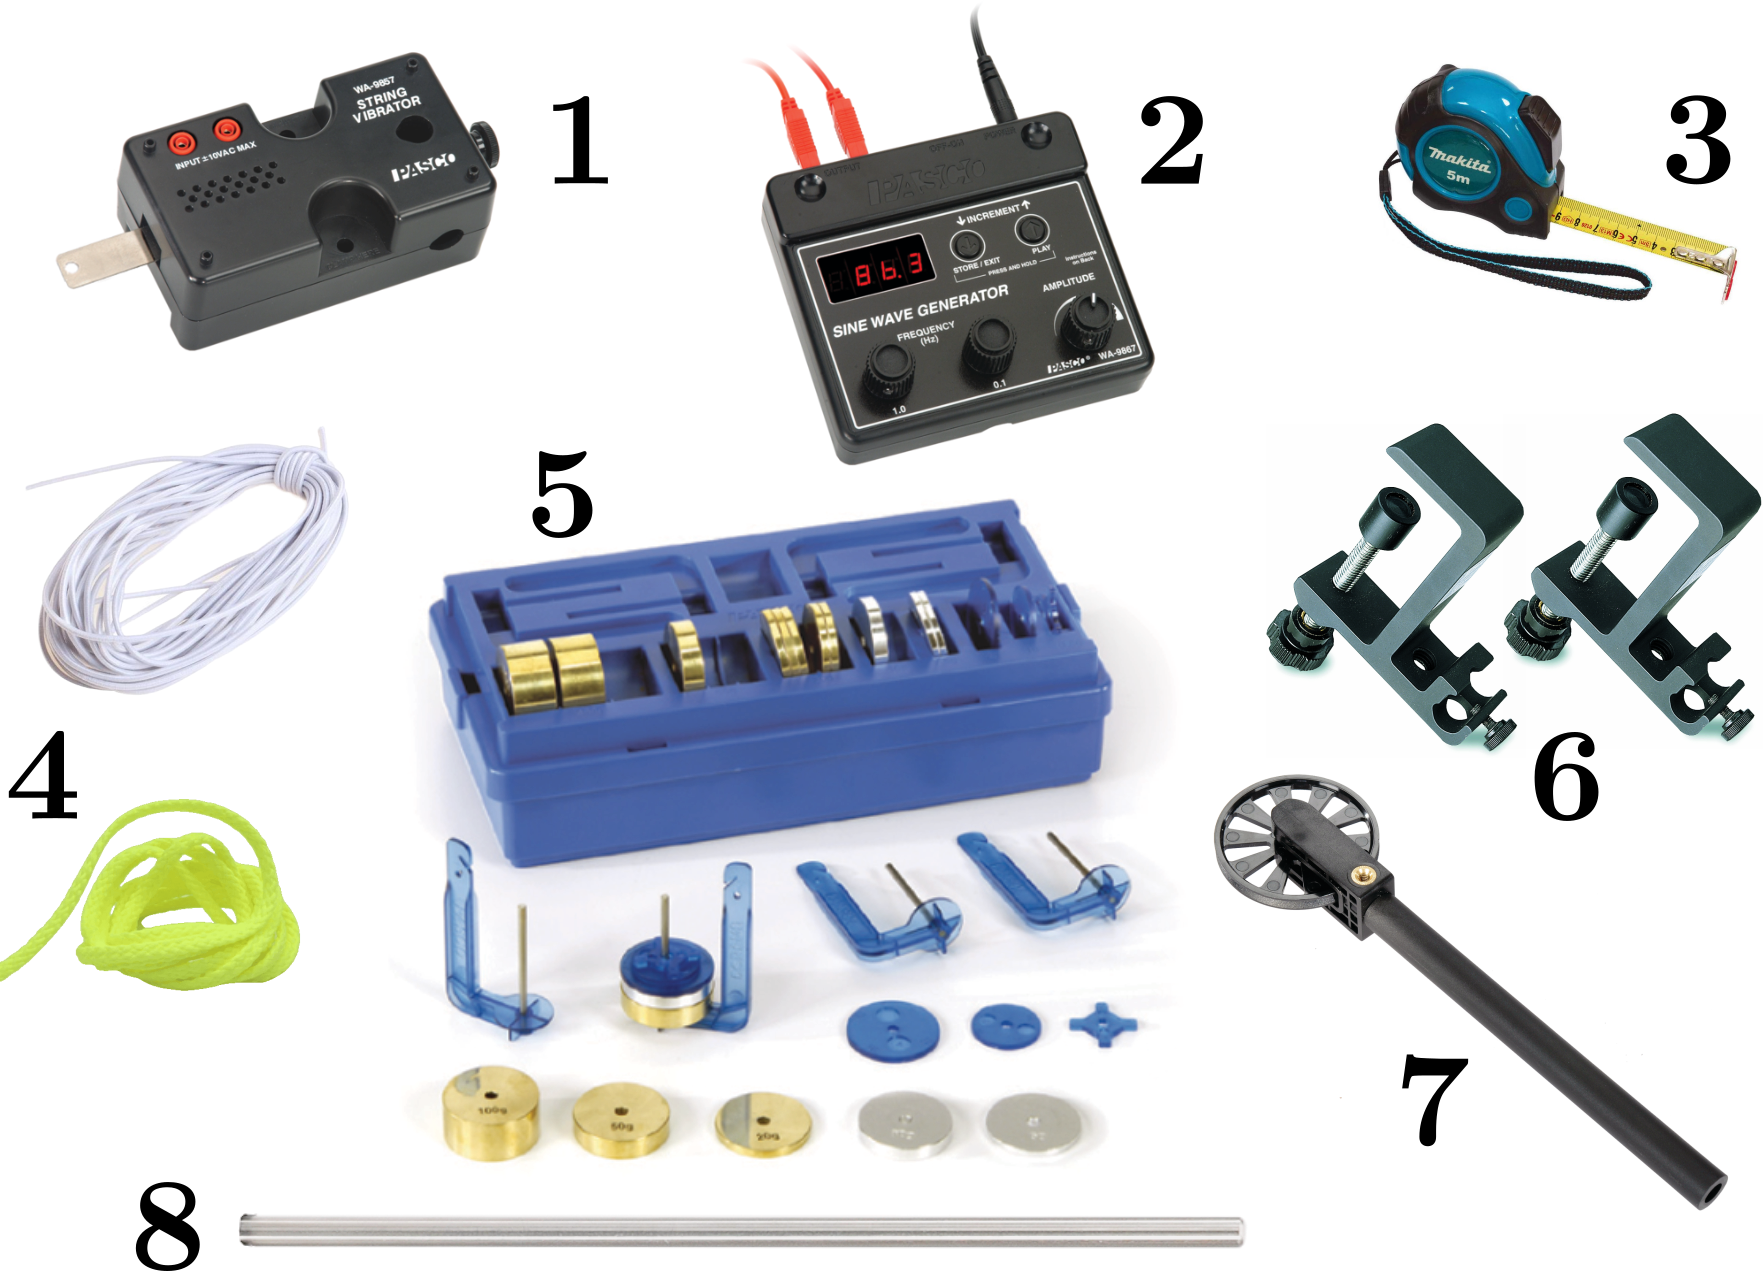
\includegraphics[width=0.5\textwidth]{station.png}
\centering
\caption{Элементы лабораторной установки}
\end{figure}

1. Механический вибратор
2. Генератор гармонических сигналов
3. Эластичная (белая) и неэластичная (зелёная) струны.
4. Рулетка
5. Набор грузов и держателей для них
6. Струбцины для крепления вибратора и опорного блока
7. Опорный блок
8. Стержень для крепления вибратора

\item Метод экспериментального исследования:

Однократный прямой замер резонансных частот.

\item Рабочие формулы:

Связь резонансной частоты с фазовой скоростью:
\begin{equation}
f_n = \frac{un}{2l}
\end{equation}

Связь фазовой скорости, силы натяжения и погонной плотности:
\begin{equation}
u = \sqrt{\frac{T}{\rho_l}}
\end{equation}


Определение погонной плотности:
\begin{equation} \label{eq:1}
\rho_l = \frac{m}{l}
\end{equation}

\item Измерительные приборы:

\begin{table}[H]
\centering
\begin{tabular}{|l|l|l|l|l|}
\hline
№ п/п & Наименование & Тип & Используемый диапазон & Погрешность приб.\\
\hline
1 & Ген. гармонич. колебаний & Электронный & 0 - 200 Гц  & 0.05 Гц\\
\hline
2 & Рулетка & Ручной & 0 - 500 см & 0.1 см\\
\hline
3 & Весы лабораторные & Ручной & 0 - 311 г. & 0.01 г.\\
\hline
\end{tabular}
\end{table}

\end{enumerate}
\section{Результаты измерений и их обработка}

Измерим длину и массу обеих струн и найдём действительную погонную плотность $\rho_l$ с учётом погрешности:


\begin{table}[H]
\begin{center}
\begin{tabular}{|c|c|c|c|c|}
\hline 
Струна & $l$, см & $m$, г & $\rho_l$, г/см & $\Delta\rho_l$, г/см \\ 
\hline 
Эластичная & 198.20 & 8.47 & 0.0427 & 0.0001\\ 
\hline 
Неэластичная & 143.40 & 2.44 & 0.0170 & 0.0001\\ 
\hline 

\end{tabular}
\caption{Результаты прямых измерений параметров струн и вычисления их погонной плотности.}
\label{tab:1}
\end{center}
\end{table}

Измерим величину резонансных частот для $n=4$ гармоники у обеих струн при различных значениях сил натяжения:

\begin{table}[H]
\begin{center}
\begin{tabular}{|c|c|c|c|c|c|c|c|}
\hline 
\multicolumn{4}{|c|}{Эластичная струна} & \multicolumn{4}{|c|}{Неэластичная струна}\\ 
\hline 
$m$, г & $f$, Гц & $f^2$, $\text{Гц}^2$ & $T$, Н & $m$, г & $f$, Гц & $f^2$, $\text{Гц}^2$ & $T$, Н \\ 
\hline 
55.00 & 22.90 & 524.41 & 0.54 & 55.00 & 37.60 & 1413.76 & 0.54\\ 
\hline 
105.00 & 30.80 & 948.64 & 1.03 & 105.00 & 51.60 & 2662.56 & 1.03\\ 
\hline 
155.00 & 38.30 & 1466.89 & 1.52 & 155.00 & 62.40 & 3893.76 & 1.52\\ 
\hline 
205.00 & 44.40 & 1971.36 & 2.01 & 205.00 & 72.00 & 5184.00 & 2.01\\ 
\hline 
255.00 & 51.30 & 2631.69 & 2.50 & 255.00 & 80.10 & 6416.01 & 2.50\\ 
\hline 
\multicolumn{4}{|c|}{$\rho_l \pm \Delta \rho_l = 0.0398 \pm 0.0001 $, г/см} & \multicolumn{4}{|c|}{$\rho_l \pm \Delta \rho_l = 0.0156 \pm 0.0001 $, г/см } \\ 
\hline 

\end{tabular}
\caption{Результаты измерений резонансных частот 4-й гармоники струн при различных силах натяжения.}
\label{tab:2}
\end{center}
\end{table}

По измеренным значения построим график зависимости квадрата резонансной частоты $f^2$ от силы натяжения $T$:

\begin{figure}[H]
\centering
\begin{tikzpicture}
\begin{axis}[
	axis lines = left,
	ylabel = \(f^2(T) \text{, Гц }^2\),
	xlabel = {\( T \text{, Н}\)},
	ymin=0,	
	ymax=6500,
	xmin=0,
	xmax=3,
	grid=both,
    grid style={line width=.1pt, draw=gray!10},
    major grid style={line width=.2pt,draw=gray!50},
    minor tick num=5,
	axis x line = bottom,
	axis line style ={line width = .3pt},
	legend style={at={(0.05, 0.9)},anchor=west}
	]


\addplot[only marks, blue1, mark size =2pt, mark=square*, error bars/.cd, y dir=both, y explicit, x dir=both, x explicit, error mark options={
      blue1,
      mark size=0.4pt,
      line width=4pt
    }, error bar style={fill=blue1,scale=2, line width=1pt}] table [y = STR1_FREQSQ, y error = STR1_FREQSQ_DIFF, x = STR1_TENS,  col sep=comma] {../freqsq_by_tension.csv};

\addplot[only marks, blue3, mark size =2pt, mark=square*, error bars/.cd, y dir=both, y explicit, x dir=both, x explicit, error mark options={
      blue3,
      mark size=0.4pt,
      line width=4pt
    }, error bar style={fill=blue3,scale=2, line width=1pt}] table [y = STR2_FREQSQ, y error = STR2_FREQSQ_DIFF, x = STR2_TENS,  col sep=comma] {../freqsq_by_tension.csv};

\addplot[blue1, domain=0:3] {1004.1399453733086*x}; 
\addplot[blue3, domain=0:3] {2567.9533585591466*x}; 

\legend{,,$f^2(T)$ Эластичная струна, $f^2(T)$ Неэластичная струна}

\end{axis}
\end{tikzpicture}
\caption{Графики зависимости квадрата резонансной частоты $f^2$ от силы натяжения для 2-х струн.}
\label{gr:1}
\end{figure}

Воспользовавшись методом наименьших  квадратов найдём угловые коэффициенты $\alpha = \frac{4}{l^2 \rho_l}$:
\begin{equation*}
\begin{aligned}
\alpha_{\text{эласт}} &\approx 1004 \pm 43 \\
\alpha_{\text{неэласт}} &\approx 2568 \pm 10
\end{aligned}
\end{equation*}

А также соответствующие погонные плотности:
\begin{equation*}
\begin{aligned}
\rho_{l \text{ эласт}} &= 0.0398 \pm 0.002 \text{ г/см} \\
\rho_{l \text{ неэласт}} &= 0.0156 \pm 0.00007 \text{ г/см}
\end{aligned}
\end{equation*}


Далее, для каждого значения силы натяжения $T$ построим зависимость резонансной частоты $f_n$ от номера гармоники $n$.

\begin{table}[H]
\begin{center}
\begin{tabular}{|c|c|c|c|c|c|c|}
\hline 
\multicolumn{7}{|c|}{Эластичная струна}\\ 
\hline 
n & $f_1$, Гц & $f_2$, Гц & $f_3$, Гц & $f_4$, Гц & $f_5$, Гц & $f_6$, Гц\\ 
\hline 
1 & 9.00 & 9.40 & 10.50 & 11.30 & 12.30 & 12.90\\ 
\hline 
2 & 17.20 & 19.60 & 21.20 & 22.90 & 24.70 & 25.70\\ 
\hline 
3 & 25.40 & 28.80 & 31.50 & 34.40 & 37.30 & 40.50\\ 
\hline 
4 & 34.20 & 38.70 & 42.50 & 47.10 & 49.80 & 53.60\\ 
\hline 
5 & 43.20 & 48.20 & 52.90 & 58.50 & 62.60 & 66.70\\ 
\hline 
г. & $m_1 = 125.00$ & $m_2 = 155.00$ & $m_3 = 185.00$ & $m_4 = 215.00$ & $m_5 = 245.00$ & $m_6 = 275.00$\\ 
\hline 
Н & $T_1 = 1.23$ & $T_2 = 1.52$ & $T_3 = 1.82$ & $T_4 = 2.11$ & $T_5 = 2.41$ & $T_6 = 2.70$\\ 
\hline 
м/c & $u_1 = 17.18$ & $u_2 = 19.30$ & $u_3 = 21.16$ & $u_4 = 23.32$ & $u_5 = 24.94$ & $u_6 = 26.68$\\ 
\hline 

\end{tabular}
\caption{Результаты измерений резонансных частот при различных номерах гармоник для \textbf{эластичной струны}.}
\label{tab:3}
\end{center}
\end{table}



\begin{table}[H]
\begin{center}
\begin{tabular}{|c|c|c|c|c|c|c|}
\hline 
\multicolumn{7}{|c|}{Неэластичная струна}\\ 
\hline 
n & $f_1$, Гц & $f_2$, Гц & $f_3$, Гц & $f_4$, Гц & $f_5$, Гц & $f_6$, Гц\\ 
\hline 
1 & 13.80 & 15.50 & 17.00 & 18.30 & 19.60 & 20.90\\ 
\hline 
2 & 28.80 & 31.60 & 33.80 & 36.80 & 39.00 & 44.10\\ 
\hline 
3 & 41.80 & 49.20 & 51.00 & 54.90 & 58.80 & 62.20\\ 
\hline 
4 & 55.80 & 62.50 & 68.30 & 73.40 & 78.40 & 85.10\\ 
\hline 
5 & 70.40 & 78.50 & 85.40 & 92.00 & 98.20 & 104.00\\ 
\hline 
г. & $m_1 = 125.00$ & $m_2 = 155.00$ & $m_3 = 185.00$ & $m_4 = 215.00$ & $m_5 = 245.00$ & $m_6 = 275.00$\\ 
\hline 
Н & $T_1 = 1.23$ & $T_2 = 1.52$ & $T_3 = 1.82$ & $T_4 = 2.11$ & $T_5 = 2.41$ & $T_6 = 2.70$\\ 
\hline 
м/c & $u_1 = 28.07$ & $u_2 = 31.59$ & $u_3 = 34.10$ & $u_4 = 36.73$ & $u_5 = 39.22$ & $u_6 = 42.04$\\ 
\hline 

\end{tabular}
\caption{Результаты измерений резонансных частот при различных номерах гармоник для \textbf{неэластичной струны}.}
\label{tab:3}
\end{center}
\end{table}


\begin{figure}[H]
\centering
\begin{tikzpicture}
\begin{axis}[
	axis lines = left,
	ylabel = \(f(T) \text{, Гц }\),
	xlabel = {\( n_{\text{гармоники}}\)},
	ymin=0,	
	ymax=110,
	xmin=1,
	xmax=6,
	grid=both,
    grid style={line width=.1pt, draw=gray!10},
    major grid style={line width=.2pt,draw=gray!50},
    minor tick num=5,
	axis x line = bottom,
	axis line style ={line width = .3pt},
	legend style={at={(0.05, 0.7)},anchor=west}
	]

\addplot[only marks, blue1, mark size =2pt, mark=square*, error bars/.cd, y dir=both, y explicit, x dir=both, x explicit, error mark options={ blue1,mark size=0.4pt, line width=4pt }, error bar style={fill=blue1,scale=2, line width=1pt}] table [y = STR1_T1, x = N,  col sep=comma] {../freq_by_harm.csv}; 
\addplot[blue1, domain=1:6] {8.589090909090908*x};
\addplot[only marks, blue2, mark size =2pt, mark=square*, error bars/.cd, y dir=both, y explicit, x dir=both, x explicit, error mark options={ blue2,mark size=0.4pt, line width=4pt }, error bar style={fill=blue2,scale=2, line width=1pt}] table [y = STR1_T2, x = N,  col sep=comma] {../freq_by_harm.csv}; 
\addplot[blue2, domain=1:6] {9.65090909090909*x};
\addplot[only marks, blue3, mark size =2pt, mark=square*, error bars/.cd, y dir=both, y explicit, x dir=both, x explicit, error mark options={ blue3,mark size=0.4pt, line width=4pt }, error bar style={fill=blue3,scale=2, line width=1pt}] table [y = STR1_T3, x = N,  col sep=comma] {../freq_by_harm.csv}; 
\addplot[blue3, domain=1:6] {10.58*x};
\addplot[only marks, blue4, mark size =2pt, mark=square*, error bars/.cd, y dir=both, y explicit, x dir=both, x explicit, error mark options={ blue4,mark size=0.4pt, line width=4pt }, error bar style={fill=blue4,scale=2, line width=1pt}] table [y = STR1_T4, x = N,  col sep=comma] {../freq_by_harm.csv}; 
\addplot[blue4, domain=1:6] {11.658181818181818*x};
\addplot[only marks, blue5, mark size =2pt, mark=square*, error bars/.cd, y dir=both, y explicit, x dir=both, x explicit, error mark options={ blue5,mark size=0.4pt, line width=4pt }, error bar style={fill=blue5,scale=2, line width=1pt}] table [y = STR1_T5, x = N,  col sep=comma] {../freq_by_harm.csv}; 
\addplot[blue5, domain=1:6] {12.469090909090909*x};
\addplot[only marks, blue6, mark size =2pt, mark=square*, error bars/.cd, y dir=both, y explicit, x dir=both, x explicit, error mark options={ blue6,mark size=0.4pt, line width=4pt }, error bar style={fill=blue6,scale=2, line width=1pt}] table [y = STR1_T6, x = N,  col sep=comma] {../freq_by_harm.csv}; 
\addplot[blue6, domain=1:6] {13.340000000000002*x};
\addplot[only marks, pink1, mark size =2pt, mark=square*, error bars/.cd, y dir=both, y explicit, x dir=both, x explicit, error mark options={ pink1,mark size=0.4pt, line width=4pt }, error bar style={fill=pink1,scale=2, line width=1pt}] table [y = STR2_T1, x = N,  col sep=comma] {../freq_by_harm.csv}; 
\addplot[pink1, domain=1:6] {14.036363636363637*x};
\addplot[only marks, pink2, mark size =2pt, mark=square*, error bars/.cd, y dir=both, y explicit, x dir=both, x explicit, error mark options={ pink2,mark size=0.4pt, line width=4pt }, error bar style={fill=pink2,scale=2, line width=1pt}] table [y = STR2_T2, x = N,  col sep=comma] {../freq_by_harm.csv}; 
\addplot[pink2, domain=1:6] {15.796363636363635*x};
\addplot[only marks, pink3, mark size =2pt, mark=square*, error bars/.cd, y dir=both, y explicit, x dir=both, x explicit, error mark options={ pink3,mark size=0.4pt, line width=4pt }, error bar style={fill=pink3,scale=2, line width=1pt}] table [y = STR2_T3, x = N,  col sep=comma] {../freq_by_harm.csv}; 
\addplot[pink3, domain=1:6] {17.05090909090909*x};
\addplot[only marks, pink4, mark size =2pt, mark=square*, error bars/.cd, y dir=both, y explicit, x dir=both, x explicit, error mark options={ pink4,mark size=0.4pt, line width=4pt }, error bar style={fill=pink4,scale=2, line width=1pt}] table [y = STR2_T4, x = N,  col sep=comma] {../freq_by_harm.csv}; 
\addplot[pink4, domain=1:6] {18.367272727272727*x};
\addplot[only marks, pink5, mark size =2pt, mark=square*, error bars/.cd, y dir=both, y explicit, x dir=both, x explicit, error mark options={ pink5,mark size=0.4pt, line width=4pt }, error bar style={fill=pink5,scale=2, line width=1pt}] table [y = STR2_T5, x = N,  col sep=comma] {../freq_by_harm.csv}; 
\addplot[pink5, domain=1:6] {19.61090909090909*x};
\addplot[only marks, pink6, mark size =2pt, mark=square*, error bars/.cd, y dir=both, y explicit, x dir=both, x explicit, error mark options={ pink6,mark size=0.4pt, line width=4pt }, error bar style={fill=pink6,scale=2, line width=1pt}] table [y = STR2_T6, x = N,  col sep=comma] {../freq_by_harm.csv}; 
\addplot[pink6, domain=1:6] {21.02*x};
\legend{,$T_{\text{эласт} 1}$, ,$T_{\text{эласт} 2}$, ,$T_{\text{эласт} 3}$, ,$T_{\text{эласт} 4}$, ,$T_{\text{эласт} 5}$, ,$T_{\text{эласт} 6}$, ,$T_{\text{неэласт} 1}$, ,$T_{\text{неэласт} 2}$, ,$T_{\text{неэласт} 3}$, ,$T_{\text{неэласт} 4}$, ,$T_{\text{неэласт} 5}$, ,$T_{\text{неэласт} 6}$}
\end{axis}
\end{tikzpicture}
\caption{Графики зависимости резонансной частоты $f$ от гармоники при различных силах натяжения для обеих струн.}
\label{gr:2}
\end{figure}

Аппроксимируем изображённые зависимости методом наименьших квадратов и получим угловые коэффициенты $\alpha = \frac{u*n}{2*l}$. С помощью этих коэффициентов построим зависимость квадрата фазовой скорости $u^2$ от силы натяжения струны $T$:


\begin{figure}[H]
\centering
\begin{tikzpicture}
\begin{axis}[
	axis lines = left,
	ylabel = \(u^2 \text{, м/с }^2\),
	xlabel = {\( T \text{, Н}\)},
	ymin=0,	
	ymax=1900,
	xmin=0,
	xmax=3,
	grid=both,
    grid style={line width=.1pt, draw=gray!10},
    major grid style={line width=.2pt,draw=gray!50},
    minor tick num=5,
	axis x line = bottom,
	axis line style ={line width = .3pt},
	legend style={at={(0.05, 0.7)},anchor=west}
	]

\addplot[only marks, blue1, mark size =2pt, mark=square*, error bars/.cd, y dir=both, y explicit, x dir=both, x explicit, error mark options={ blue1,mark size=0.4pt, line width=4pt }, error bar style={fill=blue1,scale=2, line width=1pt}] table [y = STR1_SPEED, y error = STR1_SPEED_DIFF, x = TENSION,  col sep=comma] {../speed_by_tension.csv}; 

\addplot[only marks, blue3, mark size =2pt, mark=square*, error bars/.cd, y dir=both, y explicit, x dir=both, x explicit, error mark options={ blue3,mark size=0.4pt, line width=4pt }, error bar style={fill=blue3,scale=2, line width=1pt}] table [y = STR2_SPEED, y error = STR2_SPEED_DIFF, x = TENSION,  col sep=comma] {../speed_by_tension.csv}; 
\addplot[blue1, domain=0:3] {255.81530477099787*x}; 
\addplot[blue3, domain=0:3] {645.6013983475088*x}; 

\legend{,,$u^2(T)_{\text{эласт}}$, $u^2(T)_{\text{неэласт}}$}

\end{axis}
\end{tikzpicture}
\caption{Графики зависимости квадрата фазовой  скорости $u^2$ от силы натяжения для обеих струн.}
\label{gr:2}
\end{figure}

При помощи метода наименьших квадратов найдём угловые коэффициенты $\frac{1}{\rho_l}$ графиков, а вместе с ними и погонные плотности:

\begin{equation*}
\begin{aligned}
\rho_{l \text{ эласт}} &= 0.0391 \pm 0.001 \text{ г/см} \\
\rho_{l \text{ неэласт}} &= 0.0155 \pm 0.00001 \text{ г/см}
\end{aligned}
\end{equation*}

\newpage

\section{Вывод}
Таким образом, в ходе выполнения лабораторной работы удалось, измерив резонансные частоты для эластичной и неэластичной струны при различных силах натяжения:
\begin{itemize}
\item[1.] Вычислить экспериментальные значения погонной плотности струн и сравнить их с действительными:

Для \textbf{эластичной} струны:
\begin{equation*}
\begin{aligned}
\rho_{l \text{ действительная}} &= 0.0427 \pm 0.001 \text{ г/см} \\
\rho_{l \text{ экспер. 1-метод}} &= 0.0398 \pm 0.0001 \text{ г/см} \\
\rho_{l \text{ экспер. 2-метод}} &= 0.0391 \pm 0.001 \text{ г/см} \\
\end{aligned}
\end{equation*}
Заметим, что плотности полученные экспериментальным путём довольно близки и слегка ниже полученной прямым замером (экспериментальные результаты отличаются от измеренных менее чем на $7\%$). 

Для \textbf{неэластичной} струны:
\begin{equation*}
\begin{aligned}
\rho_{l \text{ действительная}} &= 0.0170 \pm 0.0001 \text{ г/см} \\
\rho_{l \text{ экспер. 1-метод}} &= 0.0156 \pm 0.0001 \text{ г/см} \\
\rho_{l \text{ экспер. 2-метод}} &= 0.0155 \pm 0.001 \text{ г/см} \\
\end{aligned}
\end{equation*}

Для неэластичной струны результат аналогичен - экспериментальные результаты сходны, чуть меньше действительных (отличие менее $9\%$).

\item[2.] Проверить, что неэластичные струны имеют более высокие показатели резонансных частот и фазовых скоростей при одинаковых силах натяжения в сравнении с эластичными струнами. 

\end{itemize}


\section{Приложение}
Проект этой лабораторной работы, содержащий файлы с Python-кодом, использованным для вычислений и исходные TeX-файлы доступен по - \href{https://github.com/Dimankarp/Studies/tree/main/LaTeX/Physics%20-%20String%20Oscillations}{ссылке}.

\end{document}



